\section{Einführung}
\subsection{Regelkreis} \script{9}
Ein Regelkreis besteht hauptsächlich aus Aktoren, Sensoren, Regler und Kommunikation.\\
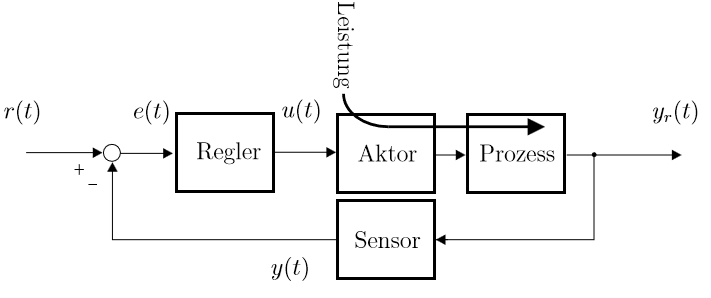
\includegraphics[width=\columnwidth]{Images/regelkreis_bsp}

\subsection{Fachwörter}
Normalerweise will man, dass die Regelgrösse der Führgrösse entspricht, dass also $y(t) = r(t)$ bzw $\varepsilon(t) = 0$ ist.\script{14}
\begin{itemize}[nosep]
	\item\underline{Festwertregelung}, wobei $r(t)$ konstant ist. Bsp: Auto B fährt mit 100m Abstand zu Auto A. Fix 100m Abstandsregelung $r(t) = 100$ was nicht über die Zeit variiert.
	\item\underline{Folgeregelung}, wobei $r(t)$ variiert mit der Zeit.
\end{itemize}
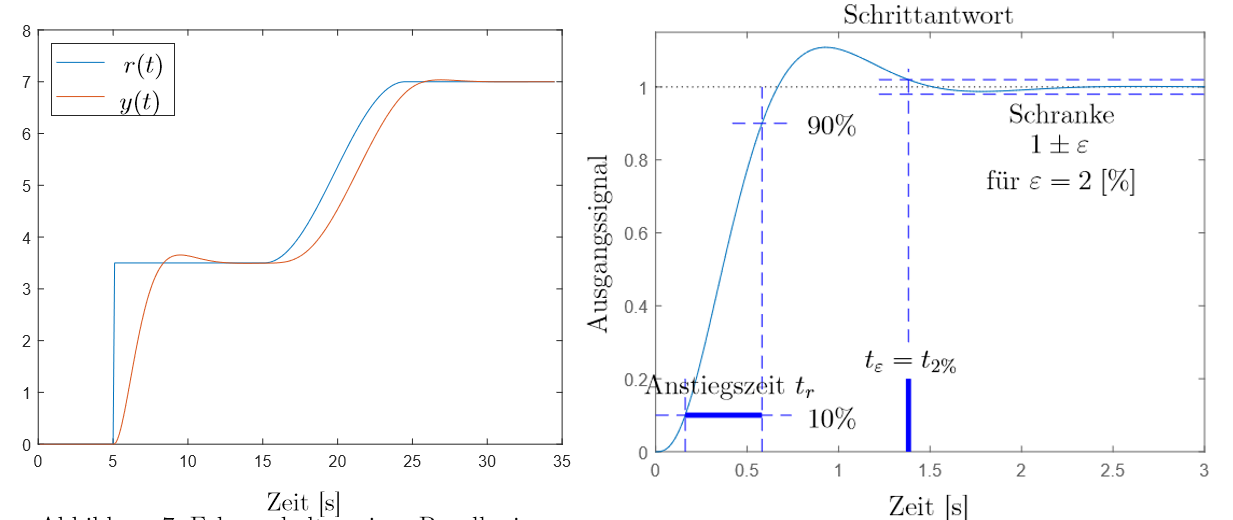
\includegraphics[width=\linewidth]{Images/regelkreis}

\begin{table}[h]
\begin{tabular}{r p{6.5cm}}
	\textbf{Steuerung:} & Reagiert nicht auf Störgrössen\\
	\textbf{Regelung:} & Aktives Feedback (zB mit Sensor), reagiert auf Störgrössen.   \\
	\textbf{Prozess:} & Entspricht einer Gesamtheit zusammenwrkender Vorgänge, durch Materie, Energie und Information umgeformt, transportiert und gespeichert wird.\\
	\textbf{System:} & ist for allem dadurch charakterisiert, dass es sich gegenüber seiner Umwelt abgrenzen lässt und klar definierte Schnittstelle zu dieser Umwelt hat. \\
	\textbf{Modell:} & schliesslich ist ein Abbildung oder eine Beschreibung, die man von einem Prozess oder einem System macht. In der Regelungstechnig verwendt man als Modelle häufig mathematische Beschreibungen wie zB Diff-Gleichungen.\\
	\textbf{Modellierung:} & von Systemen ist eine wesentliche Tätigkeit in der Regelungstechnik, denn Modelle werden für eine ganze Reihe von Zwecken benützt: sie werden herangezogen zur Erklärung, Prognose, Gestaltung oder Optimierung des Systemverhalten.
\end{tabular}
\end{table}
Weitere Fachwörter in \script{19}
